% ============================================================================
% reSTITCHing: journal extension of STITCH (MLCAD '26), v11
% ----------------------------------------------------------------------------
% The working copy of the paper. Self-contained: compiles with pdflatex alone
% ("latexmk -pdf main.tex", or one click on Overleaf) with figures/ next to
% this file. There is no supplement: the paper states everything it claims,
% and the detailed tables and figures behind it are in docs/reSTITCH.md.
%
% Figures: python -B paper/make_figures.py writes figures/*.pdf (and PNG copies
% in docs/figures/). Every number comes from the evidence files listed in
% REPO_INDEX.md; paper/V11_CHANGES.md records what changed from v10.
% Condition names in print, with their code names in the repository:
%   Baseline (baseline), Alarm (baseline_gate), Raw (raw_adv),
%   Interpret (sem_adv; v2 or v3), Escalate (sem_escalate),
%   Escalate-R (sem_escalate_restart; sem_esc_restart_v3 in the MPSoC study).
% ============================================================================
\documentclass[11pt]{article}

\usepackage[margin=1in]{geometry}
\usepackage[T1]{fontenc}
\usepackage{amsmath}
\usepackage{newtxtext,newtxmath}
\usepackage[varqu,varl,scaled=0.95]{zi4}
\usepackage{microtype}
\usepackage{graphicx}
\usepackage{xcolor}
\usepackage{booktabs,tabularx,makecell}
\usepackage{siunitx}
\usepackage{caption}
\usepackage{subcaption}
\usepackage{enumitem}
\usepackage{listings}
\usepackage{tikz}
\usetikzlibrary{arrows.meta,positioning,calc,fit}
\usepackage[section]{placeins}
\usepackage{titlesec}
\usepackage{hyperref}
\usepackage[capitalise,noabbrev,nameinlink]{cleveref}

% ---- colours: ACM link colours, and one colour per condition (paper/figstyle.py)
\definecolor{ACMPurple}{cmyk}{0.55,1,0,0.15}
\definecolor{ACMDarkBlue}{cmyk}{1,0.58,0,0.21}
\definecolor{cBase}{HTML}{8F8E89}
\definecolor{cGate}{HTML}{E3A835}
\definecolor{cRaw}{HTML}{D9622B}
\definecolor{cVtwo}{HTML}{6FA8E6}
\definecolor{cVthree}{HTML}{1D5AA6}
\definecolor{cEscP}{HTML}{63BF95}
\definecolor{cEsc}{HTML}{006E4B}
\definecolor{codebg}{HTML}{F5F4F0}
\definecolor{codeink}{HTML}{3B3A36}

\hypersetup{colorlinks=true, linkcolor=ACMPurple, citecolor=ACMPurple, urlcolor=ACMDarkBlue,
  pdftitle={reSTITCHing: Replicated, Cost-Controlled, and Sign-off-Aware Repair of LLM-Generated RTL}}
\graphicspath{{figures/}}

% ---- layout: floats stay near their first mention ---------------------------
\renewcommand{\topfraction}{0.9}
\renewcommand{\bottomfraction}{0.8}
\renewcommand{\textfraction}{0.07}
\renewcommand{\floatpagefraction}{0.8}
\setcounter{topnumber}{3}
\setcounter{bottomnumber}{2}
\setcounter{totalnumber}{4}
\setlength{\textfloatsep}{9pt plus 3pt minus 3pt}
\setlength{\floatsep}{7pt plus 2pt minus 2pt}
\setlength{\intextsep}{7pt plus 2pt minus 2pt}
\setlength{\emergencystretch}{1.5em}
\captionsetup{font=small, labelfont={bf,sf}, labelsep=period, skip=4pt}
\captionsetup[table]{position=top}
\captionsetup[sub]{font=small, labelfont={bf,sf}, skip=2pt}
% headings in the ACM journal manner: sans-serif, sections in capitals
\titleformat{\section}{\normalsize\sffamily\bfseries}{\thesection}{0.8em}{\MakeUppercase}
\titleformat{\subsection}{\normalsize\sffamily\bfseries}{\thesubsection}{0.8em}{}
\titleformat{\paragraph}[runin]{\normalsize\sffamily\bfseries}{}{0pt}{}[.]
\titlespacing*{\section}{0pt}{2.0ex plus 0.6ex minus 0.3ex}{0.8ex plus 0.2ex}
\titlespacing*{\subsection}{0pt}{1.4ex plus 0.4ex minus 0.2ex}{0.6ex plus 0.2ex}
\titlespacing*{\paragraph}{0pt}{0.9ex plus 0.3ex minus 0.2ex}{0.6em}
\setlist{itemsep=0.15em, topsep=0.3em, leftmargin=1.4em}
\sisetup{group-separator={,}, group-minimum-digits=4, retain-explicit-plus=true}
\crefname{subfigure}{Figure}{Figures}

% ---- condition names (one small-caps name each; colour swatch as in the figures)
\newcommand{\cname}[1]{\textsc{#1}}
\newcommand{\Base}{\cname{Baseline}}
\newcommand{\Alarm}{\cname{Alarm}}
\newcommand{\Raw}{\cname{Raw}}
\newcommand{\Interp}{\cname{Interpret}}
\newcommand{\Esc}{\cname{Escalate}}
\newcommand{\EscR}{\cname{Escalate-R}}
\newcommand{\Itwo}{\Interp~v2}
\newcommand{\Ithree}{\Interp~v3}
\newcommand{\sw}[1]{\textcolor{#1}{\rule[-0.12ex]{0.8em}{0.8em}}}
\newcommand{\tool}[1]{\texttt{#1}}
\newcommand{\runin}[1]{\textbf{\sffamily #1.}\ }

% ---- code and tool output -------------------------------------------------
\lstdefinestyle{rtl}{language=Verilog, basicstyle=\ttfamily\fontsize{7}{8.4}\selectfont\color{codeink},
  keywordstyle=\color{ACMDarkBlue}\bfseries, commentstyle=\color{cRaw}, columns=fullflexible,
  keepspaces=true, backgroundcolor=\color{codebg}, frame=none, xleftmargin=3pt, xrightmargin=3pt,
  aboveskip=2pt, belowskip=0pt, showstringspaces=false}
\lstdefinestyle{log}{language={}, basicstyle=\ttfamily\fontsize{6.6}{7.9}\selectfont\color{codeink},
  columns=fullflexible, keepspaces=true, breaklines=true, breakindent=1em, backgroundcolor=\color{codebg},
  frame=none, xleftmargin=3pt, xrightmargin=3pt, aboveskip=2pt, belowskip=0pt}

\title{\sffamily\bfseries reSTITCHing: Replicated, Cost-Controlled, and Sign-off-Aware\\Repair of LLM-Generated RTL}
\author{\sffamily Karthikeya Patana \and \sffamily Yashwant Rajesh \and \sffamily Aathira Sunil \and
  \sffamily Durga Saranyu \and \sffamily Sri Parameswaran \and \sffamily Kamesh Chandrasekar \and
  \sffamily Paresh Saxena \and \sffamily Soumya Joshi}
\date{}

\begin{document}
\maketitle

% ============================================================================
\begin{abstract}
\noindent Repair loops that feed simulation results back to a language model
make its Verilog pass the testbench more often, but passing simulation is not
passing sign-off: an inferred latch or a reset that synthesis cannot map
simulates correctly and surfaces only in synthesis or timing analysis. STITCH
(MLCAD~'26) adds lint and synthesis to the loop, with a deterministic
interpreter that turns their diagnostics into repair directives at no inference
cost. This article replicates its single-run evidence, adds a policy that calls
on the interpreter only when a run is stuck, and evaluates both with twelve
open and commercial models on the RTLLM benchmark and on a hand-written RISC-V
multiprocessor system-on-chip. On RTLLM the interpreter's effect on pass rate is
small and model-dependent, while the stuck-only policy keeps baseline accuracy
and saves more tool calls the stronger the model. On the multiprocessor, a
simulation-only loop accepts defective modules in nearly two-thirds of its runs,
at every model size; with STITCH, latch-free synthesisable repairs of the
latch-bearing modules rise from 24\% to 88\%. A pre-registered control shows
that the detail of the diagnosis, not the alarm that sign-off failed, drives
repair, and the repaired modules restore synthesis of 4- and 9-router networks.

\medskip
\noindent\textbf{\sffamily Keywords:} large language models, Verilog, RTL
repair, lint, logic synthesis, sign-off, inferred latches, network-on-chip
\end{abstract}

% ============================================================================
\section{Introduction}
\label{sec:intro}

Simulation answers one question about a hardware design: does it produce the
expected outputs for the inputs the testbench applies? Sign-off asks more: lint
and logic synthesis must accept the block, and static timing analysis must
close it. \Cref{fig:motivation} shows a defect that passes the first test and
fails the second, taken from the hand-written RISC-V core studied in this
article. The multiplexer chooses the next program counter from three sources.
The fourth select value never occurs in operation, so the designer left it out
of the \texttt{case} statement and the testbench never applies it. The module
passes its testbench, but synthesis must hold the output for the missing value,
and without a clock it can only do so with latches: Yosys builds $32$.

\begin{figure}[!t]
\centering
\begin{minipage}[t]{0.40\linewidth}
\textsf{\footnotesize\textbf{(a)} The RTL as written (reformatted; comment ours)}
\begin{lstlisting}[style=rtl]
module MuxPC(
  input  [31:0] next_address, B_addr, J_addr,
  input  [1:0]  PCsrc,
  output reg [31:0] input_to_ifu);
  always @(*)
    case (PCsrc)
      2'b00: input_to_ifu = next_address;
      2'b01: input_to_ifu = J_addr;
      2'b10: input_to_ifu = B_addr;
      // 2'b11 "does not occur in operation"
    endcase
endmodule
\end{lstlisting}
\end{minipage}\hfill
\begin{minipage}[t]{0.575\linewidth}
\textsf{\footnotesize\textbf{(b)} What each check reports}
\begin{lstlisting}[style=log]
Simulation  PASS   (the testbench never applies PCsrc = 2'b11)
Verilator   %Warning-CASEINCOMPLETE: Case values incompletely covered
            (example pattern 0x3)
Yosys       Latch inferred for signal `\MuxPC.\input_to_ifu' ...
            $_DLATCH_N_   32
\end{lstlisting}
\vspace{3pt}
\textsf{\footnotesize\textbf{(c)} The STITCH directive (abridged)}
\begin{lstlisting}[style=log]
*** YOSYS: LATCH INFERRED for signal(s) 'input_to_ifu' ***
ROOT CAUSE: Yosys inferred a latch on 'input_to_ifu' because it is not
assigned on every code path through the always block. [...]
EXACT FIX: Add a default branch to the case that assigns 'input_to_ifu':
    default: input_to_ifu = <safe value>;   <-- ADD THIS
\end{lstlisting}
\end{minipage}
\caption{A sign-off defect that simulation cannot see, from the hand-written
MPSoC of \cref{sec:mpsoc}. (a)~The next-PC multiplexer omits a select value
that never occurs in operation. (b)~It passes its testbench, but synthesis
infers $32$ latches. (c)~STITCH turns the tool output into a directive that
names the signal and the fix. Tool messages are quoted, abridged, from
Verilator~5.020 and Yosys~0.33.}
\label{fig:motivation}
\end{figure}

An inferred latch is not cosmetic. Its enable is decoded by combinational
logic, so a glitch can open it and capture a wrong value; timing analysis must
time paths through a level-sensitive element nobody intended, so a block that
simulates perfectly can still fail timing; and test insertion cannot scan it as
it would a flip-flop. Incomplete \texttt{case} statements are a textbook source
of such latches and of mismatches between simulation and
synthesis~\cite{cummings1999}. Other defect classes share the blind spot: a net
with two drivers; an asynchronous reset written in a form synthesis cannot map,
which simulates as intended and then aborts synthesis; and a width mismatch
that silently drops the high bits of a bus.

Large language models now write Verilog from natural-language
specifications~\cite{verilogeval,lu2024rtllm}, and repair loops such as
AutoChip~\cite{autochip} feed the simulator's verdict back to the model until
the testbench passes. Such a loop stops exactly when these defects become
invisible, and delivers them with the code. STITCH, introduced in our
conference paper~\cite{stitch26}, adds the two checks a sign-off flow runs
first, Verilator lint~\cite{verilator} and Yosys synthesis~\cite{yosys}, and
places a deterministic interpreter between them and the model. The interpreter
rewrites a raw diagnostic as a short directive that names the signal and the
fix (\cref{fig:motivation}c); it is a fixed set of rules and costs no model
call.

The conference paper illustrated four ways the interpreter can affect a run
(enabling a repair, protecting a model from confusing raw tool text, harming a
run that was converging, or being irrelevant), each with a single run. One run
cannot separate a mechanism from luck, and modules written for a study say
little about real hardware. We therefore ask: which effects survive
replication; when does the interpreter help, and at what cost; do the answers
hold from small open models to commercial ones; and does any of it matter on a
design written by engineers rather than by the study?

For the last question we use a RISC-V multiprocessor system-on-chip (MPSoC)
written by hand within our group for an earlier project, independently of this
study: five-stage RV32 cores connected through network interfaces to a mesh
network-on-chip of $4$ or $9$ routers. Open-source synthesis of it reports $63$
latch inferences and then aborts on a reset it cannot map. Its defects are
natural rather than seeded, they sit in small leaf modules that are
instantiated many times, and they let us ask what no module-level benchmark
can: does repairing the leaves let the whole design synthesise?
\Cref{fig:teaser} previews the answer.

\begin{figure}[!t]
\centering
\begin{subfigure}[t]{2.08in}
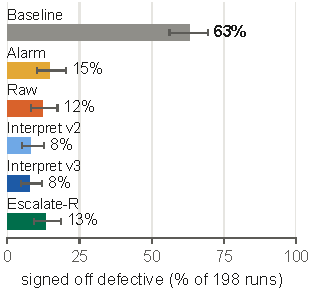
\includegraphics{fig_teaser_a}
\caption{Signed off defective}
\label{fig:teaser-a}
\end{subfigure}\hfill
\begin{subfigure}[t]{2.08in}
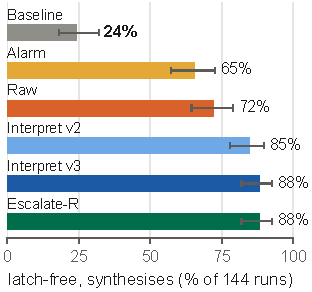
\includegraphics{fig_teaser_b}
\caption{Latch-bearing tasks}
\label{fig:teaser-b}
\end{subfigure}\hfill
\begin{subfigure}[t]{2.08in}
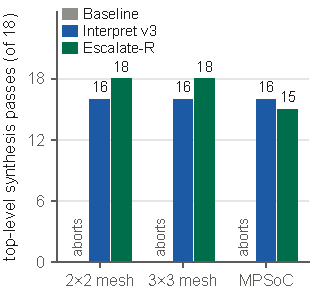
\includegraphics{fig_teaser_c}
\caption{Top-level synthesis restored}
\label{fig:teaser-c}
\end{subfigure}
\caption{STITCH on the hand-written MPSoC (six open models, $198$ runs per
condition; conditions in \cref{tab:conditions}). (a)~Simulation-only repair
signs off $63\%$ of its runs as defective. (b)~On the eight latch-bearing tasks,
runs that end latch-free with a clean synthesis rise from $24\%$ to $88\%$.
(c)~With the repaired modules spliced back, simulation-only repair never yields
a design that synthesises; \Ithree{} and \EscR{} do in $15$ to $18$ of $18$
attempts.}
\label{fig:teaser}
\end{figure}

\paragraph{Claims} Each rests on three replicated runs per configuration and on a
check that the interpreter fired in every run credited to it.
\begin{enumerate}[label=\textbf{\sffamily C\arabic*.}, leftmargin=2.1em, itemsep=0.15em]
\item \textbf{Simulation-only repair signs off defective hardware at every model
size}: $63\%$ of its MPSoC runs, including every simulation-silent defect for
every model; with lint and synthesis in the loop, $8$ to $15\%$
(\cref{sec:mpsoc-results}).
\item \textbf{The diagnosis, not the alarm, drives repair.} A pre-registered
control that only says sign-off failed does no better than raw tool output;
escalating to the interpreter lifts sign-off-clean runs from $52$ to $72\%$
(\cref{sec:mpsoc-results}).
\item \textbf{Module-level repairs compose}: the repaired modules restore
synthesis of both meshes and the MPSoC top, which simulation-only repair never
does (\cref{sec:mpsoc-results}).
\item \textbf{Escalating only when a run is stuck preserves baseline accuracy (with
one restart allowed) and saves tool calls}: escalation calls lint and synthesis
$17\%$ less often than always-on interpretation on small open models, and $89\%$
less on commercial ones (\cref{sec:escalation,sec:rtllm}).
\item \textbf{On a testbench-scored benchmark the interpreter's pass-rate effect
is small and model-dependent}, and only replication shows it: two conference
illustrations replicate; three larger candidates, and two of our own first
readings (a harmful effect at scale, an escalation win on larger models), do not
(\cref{sec:replication,sec:rtllm}).
\end{enumerate}

\paragraph{Relation to the conference version} The conference
paper~\cite{stitch26} introduced the lint and synthesis layer, the interpreter,
a $20$-module in-house suite and the four outcome types (recapped in
\cref{sec:stitch}); everything else here is new. Two readings are revised: the
harmful effect survives only as a non-significant deficit on small models, and
failures with no tool-visible signal are, on RTLLM's hardest modules, mostly
beyond small open models rather than beyond the tools.

% ============================================================================
\section{Related Work}
\label{sec:related}

\paragraph{Benchmarks and fine-tuned generators} VerilogEval~\cite{verilogeval}
and RTLLM~\cite{lu2024rtllm} score generated RTL against reference testbenches;
we use RTLLM~v2.1. RTLCoder~\cite{rtlcoder} fine-tunes a code model on curated
Verilog from the same weights as DeepSeek-Coder~\cite{deepseekcoder}, so the
pair isolates fine-tuning (\cref{sec:finetune}).

\paragraph{Feedback loops and agents} Self-Refine~\cite{selfrefine} established
iterative refinement with self-generated feedback. AutoChip~\cite{autochip}
feeds compilation errors and simulation mismatches back to the model,
RTLFixer~\cite{rtlfixer} repairs syntax errors from compiler feedback, and Qiu
et al.~\cite{qiu2024} use language models to explain EDA tool errors. Agentic
systems add planners, waveform tracers, checkpoints or UVM testing around
several model calls: VerilogCoder~\cite{verilogcoder}, MAGE~\cite{mage},
AIvril~\cite{aivril}, MEIC~\cite{meic} and UVLLM~\cite{uvllm}. STITCH is
orthogonal: it changes what is fed back (lint and synthesis diagnostics,
translated deterministically, with no extra model call), and we evaluate it
with replication, by difficulty tier, against a sign-off oracle the loop never
sees, and with a control that separates being told \emph{that} a check failed
from being told \emph{what} failed.

% ============================================================================
\section{STITCH and the Feedback Conditions}
\label{sec:stitch}

\Cref{fig:pipeline} shows the loop. In each iteration the model returns RTL,
Icarus Verilog~\cite{iverilog} simulates it against the \emph{loop testbench},
and on a failure the loop feeds back the simulation log and, depending on the
condition, the Verilator and Yosys output, raw or interpreted.

\begin{figure}[!htbp]
\centering
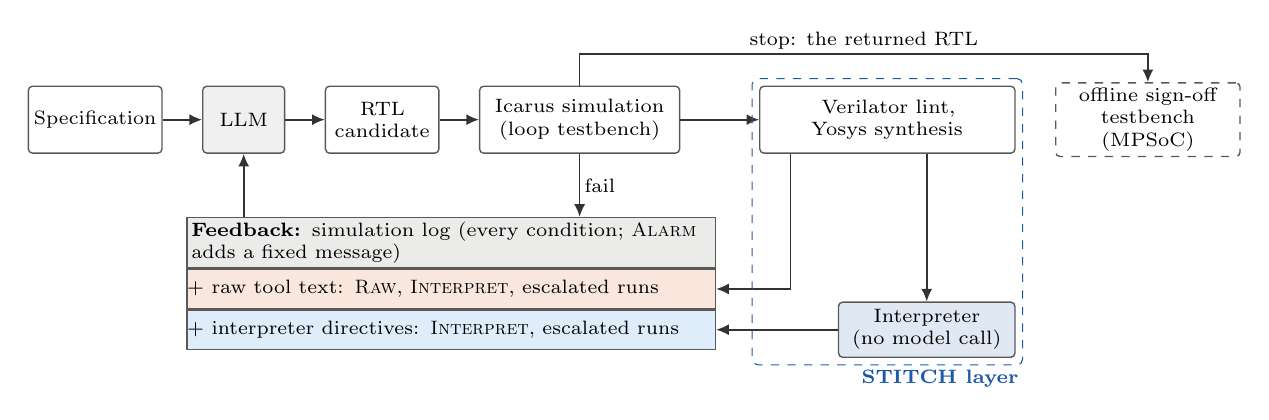
\begin{tikzpicture}[font=\scriptsize, >={Latex[length=1.6mm,width=1.4mm]},
  box/.style={draw=black!65, rounded corners=1.5pt, align=center, minimum height=8.5mm, inner sep=2pt, line width=0.5pt},
  part/.style={draw=black!65, align=left, text width=66mm, minimum height=5mm, inner sep=1.6pt, font=\scriptsize, line width=0.5pt},
  arr/.style={->, line width=0.6pt, draw=black!80},
  lab/.style={font=\scriptsize, inner sep=1.5pt}]
\node[box] (spec) {Specification};
\node[box, text width=9mm, fill=black!6, right=5mm of spec] (llm) {LLM};
\node[box, text width=13mm, right=5mm of llm] (rtl) {RTL\\candidate};
\node[box, text width=24mm, right=5mm of rtl] (sim) {Icarus simulation\\(loop testbench)};
\node[box, text width=31mm, right=10mm of sim] (tools) {Verilator lint,\\Yosys synthesis};
\node[box, dashed, text width=22mm, right=5mm of tools] (sign) {offline sign-off\\testbench (MPSoC)};
\node[part, fill=cBase!18, anchor=north west] (f1) at ($(llm.south west)+(-2mm,-8mm)$) {\textbf{Feedback:} simulation log (every condition; \Alarm{} adds a fixed message)};
\node[part, fill=cRaw!16, below=0pt of f1] (f2) {+ raw tool text: \Raw, \Interp, escalated runs};
\node[part, fill=cVtwo!22, below=0pt of f2] (f3) {+ interpreter directives: \Interp, escalated runs};
\node[box, text width=21mm, minimum height=7mm, fill=cVthree!14, anchor=east] (interp) at (tools.east |- f3) {Interpreter\\(no model call)};
\draw[arr] (spec) -- (llm);
\draw[arr] (llm) -- (rtl);
\draw[arr] (rtl) -- (sim);
\draw[arr] (sim) -- (tools);
\draw[arr] (sim.south) -- node[right, lab]{fail} (sim.south |- f1.north);
\draw[arr] ($(tools.south west)+(4mm,0)$) |- (f2.east);
\draw[arr] (interp.north |- tools.south) -- (interp.north);
\draw[arr] (interp.west) -- (f3.east);
\draw[arr] (llm.south |- f1.north) -- (llm.south);
\draw[arr] (sim.north) -- ++(0,4mm) -| node[pos=0.25, above, lab]{stop: the returned RTL} (sign.north);
\node[draw=cVthree, dashed, rounded corners=2pt, inner sep=2.5pt, fit=(tools)(interp)] (stitch) {};
\node[font=\scriptsize\bfseries, text=cVthree, anchor=north east, inner sep=1.5pt] at (stitch.south east) {STITCH layer};
\end{tikzpicture}
\caption{The STITCH loop. What is fed back after a failing iteration depends on
the condition (\cref{tab:conditions}). In the MPSoC study a
specification-complete sign-off testbench scores the returned RTL offline and
never reaches the loop.}
\label{fig:pipeline}
\end{figure}

\paragraph{The interpreter} The interpreter (\cref{tab:rules}) is a fixed rule
set that maps each diagnostic it recognises to a directive naming the signal and
the fix, and calls no model. Version v2 is the production interpreter of the
conference paper and runs unchanged in every study. Version v3 is an additive
layer written during the MPSoC study (\cref{sec:mpsoc-design}): it reproduces
v2 byte for byte wherever none of its four new rules applies.

\begin{table}[!htbp]
\centering
\footnotesize
\caption{Interpreter rule classes. v2 is the production interpreter; v3 adds
four rules found necessary on the MPSoC's real tool logs.}
\label{tab:rules}
\begin{tabularx}{\linewidth}{@{}l l X@{}}
\toprule
Class & Source & Directive, in short \\
\midrule
\multicolumn{3}{@{}l}{\emph{v2 (production)}} \\
\tool{UNUSEDSIGNAL} & Verilator & a declared input is never read: use it (e.g.\ gate the output on it) \\
\tool{MULTIDRIVEN} & Verilator & a signal has several drivers: keep one \\
\tool{UNDRIVEN} & Verilator & an output is never assigned, or a name is undeclared \\
\tool{WIDTHTRUNC/EXPAND} & Verilator & a width mismatch on an assignment: size the operands \\
\tool{BLKSEQ}, \tool{COMBDLY} & Verilator & blocking or delayed assignment in the wrong block type \\
Latch inferred & Yosys & assign every output on every path of the block \\
Combinational loop & Yosys & break the feedback path \\
\addlinespace
\multicolumn{3}{@{}l}{\emph{v3 additions}} \\
\tool{MISSING\_CLOCK} & both & a Yosys latch in a level-sensitive block plus an unused clock: make the block edge-triggered \\
\tool{ASYNC\_RESET} & Yosys & ``multiple edge sensitive events'' abort: one asynchronous reset, other clears synchronous \\
\tool{WIDTH\_EXPR} & Verilator & a width warning on an expression, which v2 dropped \\
\tool{COMB\_LOOP} & Verilator & a loop Verilator reports (\tool{UNOPTFLAT}) when Yosys reports none \\
\bottomrule
\end{tabularx}
\end{table}

\paragraph{Feedback conditions} All conditions share the prompt and the budget
and differ only in what is fed back after a failing iteration
(\cref{tab:conditions}). \Alarm, a control used in the MPSoC study, says
\emph{that} sign-off failed but never \emph{what} failed. The same colour marks
each condition in every figure.

\begin{table}[!htbp]
\centering
\footnotesize
\caption{The feedback conditions and their colours in the figures. All see the
simulation log. On RTLLM every run stops at its first testbench pass; in the
MPSoC study \Base{} stops at its first simulation pass, as AutoChip does, and
every other condition at its first pass that is also lint- and synthesis-clean.}
\label{tab:conditions}
\begin{tabularx}{\linewidth}{@{}c l X l@{}}
\toprule
 & Condition & Fed back after a failing iteration, besides the simulation log & Used in \\
\midrule
\sw{cBase}   & \Base   & nothing (the AutoChip loop) & all studies \\
\sw{cGate}   & \Alarm  & a fixed message: ``the design simulates correctly but fails synthesis sign-off'' & MPSoC \\
\sw{cRaw}    & \Raw    & the raw Verilator and Yosys text & in-house, MPSoC \\
\sw{cVtwo}\,\sw{cVthree} & \Interp & the raw text and the interpreter's directives, on every iteration (v2; in the MPSoC study, v2 or v3) & all but tiering \\
\sw{cEscP}   & \Esc    & nothing until the run is stuck, then what \Interp{} feeds back, for the rest of the run & in-house, RTLLM \\
\sw{cEsc}    & \EscR   & as \Esc, plus one restart from a blank prompt if the run stays stuck & all but tiering \\
\bottomrule
\end{tabularx}
\end{table}

\subsection{Escalating Only When a Run Is Stuck}
\label{sec:escalation}

Feeding directives on every iteration intervenes even when nothing is wrong,
and can derail a run that was converging. Escalation intervenes only once a run
is stuck (\cref{fig:esc}). Each failure yields an error signature, the first
five lines of the normalised log. After two consecutive failures with the same
signature, the run switches for good to what \Interp{} feeds back; \EscR{} also
restarts once from a blank prompt after three further same-signature failures.

\begin{figure}[!htbp]
\centering
\begin{minipage}[t]{0.52\linewidth}
\centering
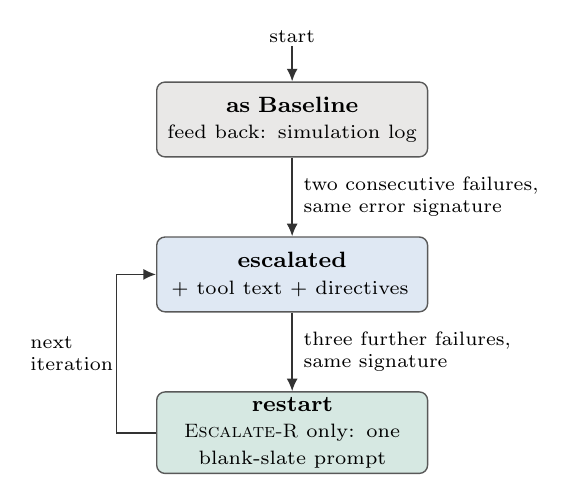
\begin{tikzpicture}[baseline=(current bounding box.north), font=\footnotesize, >={Latex[length=1.6mm,width=1.4mm]},
  st/.style={draw=black!65, rounded corners=3pt, align=center, text width=33mm, minimum height=9.5mm, inner sep=2pt, line width=0.5pt},
  arr/.style={->, line width=0.6pt, draw=black!80},
  lab/.style={font=\scriptsize, align=left, inner sep=1pt}]
\node[st, fill=cBase!20] (b) {\textbf{as \Base}\\{\scriptsize feed back: simulation log}};
\node[st, fill=cVthree!14, below=10mm of b] (e) {\textbf{escalated}\\{\scriptsize + tool text + directives}};
\node[st, fill=cEsc!16, below=10mm of e] (r) {\textbf{restart}\\{\scriptsize \EscR{} only: one blank-slate prompt}};
\draw[arr] ($(b.north)+(0,4.5mm)$) node[above, lab]{start} -- (b.north);
\draw[arr] (b.south) -- node[right, lab, xshift=1mm]{two consecutive failures,\\same error signature} (e.north);
\draw[arr] (e.south) -- node[right, lab, xshift=1mm]{three further failures,\\same signature} (r.north);
\draw[arr] (r.west) -- ++(-5mm,0) |- node[pos=0.25, left, lab]{next\\iteration} (e.west);
\end{tikzpicture}
\captionof{figure}{The escalation policies. A pass stops the run in any state;
until the first trigger, an escalation run is a \Base{} run.}
\label{fig:esc}
\end{minipage}\hfill
\begin{minipage}[t]{0.44\linewidth}
\centering
\footnotesize
\captionof{table}{Cost per run on the $255$-run in-house benchmark: escalation
calls the heavyweight tools least.}
\label{tab:cost}
\begin{tabular}{@{}l r r@{}}
\toprule
Condition & \makecell[r]{Tokens\\per run} & \makecell[r]{Tool calls\\per run} \\
\midrule
\sw{cBase}\ \Base   & 4,891 & 0.00 \\
\sw{cRaw}\ \Raw     & 5,354 & 2.61 \\
\sw{cVtwo}\ \Interp & 4,883 & 2.37 \\
\sw{cEscP}\ \Esc    & 5,151 & \textbf{1.53} \\
\sw{cEsc}\ \EscR    & 4,719 & \textbf{1.37} \\
\bottomrule
\end{tabular}
\end{minipage}
\end{figure}

Until the trigger, an escalation run is a \Base{} run, so \emph{on every run that
converges before the trigger, escalation is the baseline policy}; beyond it,
nothing guarantees baseline accuracy, and \cref{sec:small} tests it. On a
$255$-run benchmark of the conference paper's in-house modules ($17$ model and
module pairs, five conditions, three runs each), escalation calls Verilator and
Yosys $35$ to $45\%$ less often than \Raw{} and \Interp{} at a matching or
better pass rate (\cref{tab:cost}). Tokens can rise, because escalated runs use
extra iterations, so our efficiency claims refer to tool calls.

% ============================================================================
\section{Experimental Method}
\label{sec:method}

\subsection{Studies and Models}
\label{sec:studies}

Besides the in-house replication (\cref{sec:replication}), we ran five studies
(\cref{tab:studies}). Four use RTLLM~v2.1~\cite{lu2024rtllm}, a public benchmark
of module specifications with reference testbenches: the first runs \Base{}
only, to tier the modules (\cref{sec:tiers}) and to test fine-tuning
(\cref{sec:finetune}), and the next three compare conditions on small open,
larger open and commercial models. The fifth is the MPSoC case study. Open
models ran quantised, served by Ollama~\cite{ollama} on the institutional GPU
cluster; commercial models ran through their APIs with reasoning disabled and
the same runner code, prompts and toolchain.

\begin{table}[!htbp]
\centering
\footnotesize
\caption{The five studies. A dot marks a model that ran in the study;
swatches as in \cref{tab:conditions}. Every configuration ran three times.}
\label{tab:studies}
\setlength{\tabcolsep}{4pt}
\newcommand{\y}{$\bullet$}
\begin{tabular}{@{}l ccccc@{}}
\toprule
 & \makecell{Tiering and\\fine-tuning} & \makecell{Small open\\models} & \makecell{Larger open\\models} & \makecell{Commercial\\models} & \makecell{MPSoC\\case study} \\
\midrule
\multicolumn{6}{@{}l}{\emph{Open models, served locally}} \\
Llama~3.2 3B~\cite{llama3}            &    &    &    &    & \y \\
Gemma~3 4B~\cite{gemma3}              & \y & \y &    &    & \y \\
DeepSeek-Coder 6.7B~\cite{deepseekcoder} & \y & \y &    &    & \y \\
RTLCoder 6.7B~\cite{rtlcoder,rtlcoder_hf}, two prompts & \y &    &    &    &    \\
Qwen2.5-Coder 7B~\cite{qwen25coder}   &    &    &    &    & \y \\
Llama~3.1 8B~\cite{llama3}            & \y & \y &    &    & \y \\
Qwen2.5-Coder 14B~\cite{qwen25coder}  &    &    & \y &    & \y \\
Gemma~3 27B~\cite{gemma3}             &    &    & \y &    &    \\
Qwen2.5-Coder 32B~\cite{qwen25coder}  &    &    & \y &    & \y \\
\multicolumn{6}{@{}l}{\emph{Commercial models, through their APIs, without reasoning}} \\
GPT-4.1 mini                          &    &    &    & \y & \y \\
Gemini~2.5 Flash                      &    &    &    & \y & \y \\
Claude Haiku~4.5                      &    &    &    & \y & \y \\
\midrule
Tasks & 42 RTLLM & 42 RTLLM & 17 recoverable & \makecell{17 recoverable,\\19 floor} & 11 MPSoC \\
\addlinespace[2pt]
Conditions & \sw{cBase} & \sw{cBase}\,\sw{cVtwo}\,\sw{cEscP}\,\sw{cEsc} & \sw{cBase}\,\sw{cVtwo}\,\sw{cEscP}\,\sw{cEsc} & \sw{cBase}\,\sw{cVtwo}\,\sw{cEscP}\,\sw{cEsc} & \sw{cBase}\,\sw{cGate}\,\sw{cRaw}\,\sw{cVtwo}\,\sw{cVthree}\,\sw{cEsc} \\
\addlinespace[2pt]
Temperature & 0.5 & 0.1 & 0.1 & 0.1 & 0.1 \\
Runs & 630 & 1,512 & 612 & 1,211 & 1,980 \\
\bottomrule
\end{tabular}
\end{table}

\subsection{Replication and Statistics}
\label{sec:stats}

Every configuration (a model, a module or task, and a condition) is run three
times. Three runs separate a unanimous outcome ($3/3$ or $0/3$) from a split
and expose a single-run ``win'' as sampling noise, at a cost that stays
affordable over thousands of runs; the price is that small per-model effects
remain undecided, and we say so where it matters. A rate carries a Wilson $95\%$
interval~\cite{wilson1927}. A difference between two conditions is computed
within each (model, module) cell and averaged over cells; because the three
runs of a cell share a model and a module, its interval comes from resampling
whole cells (a bootstrap) and its $p$-value from a sign-flip test over cells. A
difference is significant when its $95\%$ interval excludes zero. No pass is
credited to the interpreter unless the interpreter actually fired in that run.

\subsection{A Harness That Cannot Fail Silently}
\label{sec:harness}

We found and fixed three silent defects in the shared runner. The simulator ran
without a working directory, so a testbench that loads a data file could never
pass; unclosed code fences corrupted $58$ of $659$ generated files ($8.8\%$);
and the pass check looked for \texttt{"PASS"} while RTLLM testbenches print
\texttt{"Your Design Passed"}, so $20$ of $64$ completed runs ($31\%$) were
misclassified as failures and spent their remaining iterations ``fixing''
correct code. All three are one fragility, an assumption about a benchmark's
output buried in shared code, so every result here routes pass detection
through one function backed by a per-benchmark registry with no default: an
unregistered benchmark fails at once rather than silently.

% ============================================================================
\section{Replication: What Survives Three Runs}
\label{sec:replication}

The conference paper's cleanest illustration, a gating input that the model
declares but never reads, replicates in all three runs on two modules,
\texttt{decoder\_3to8} and \texttt{mux4\_oe}. Verilator reports the unused
input and the directive names the port. Gemma~3 4B then passes in two
iterations, where under \Base{} and \Raw{} it fails all six in every run;
Llama~3.1 8B passes under all three conditions. \Raw{} tracks \Base{} exactly,
so the effect comes from the interpretation, not from the presence of the
tools.

\paragraph{A reachability asymmetry} A forgotten \emph{input} reliably produces
the target defect, but a forgotten \emph{output} does not: on the two modules
built for it, Gemma~3 4B assigned every declared output unprompted, so the
interpreter correctly had nothing to fire on. Driving a declared output is a
local obligation a model closes by itself; reading a declared input is a
non-local one, and a module that ignores an input still compiles and looks
complete. Which defects the interpreter can reach depends on how the model
fails, and has to be measured per defect class.

\paragraph{What replication retired} Three larger candidates built to show the
mechanism at scale did not survive. On \texttt{datapath\_mux\_alu}, Llama~3.1 8B
passed under \Interp{} in $2$ of $3$ runs without the interpreter ever firing: a
single run would have read as a win. On \texttt{instr\_decode\_unit}, Gemma~3 4B
received the correct directive and still failed, in a syntax loop; and
\texttt{alu\_with\_enable} became too easy after its redesign. Likewise, six of
eight in-house benchmark cells labelled from a single run did not reproduce
their label with three.

% ============================================================================
\section{STITCH on RTLLM}
\label{sec:rtllm}

\subsection{Benchmark and Difficulty Tiers}
\label{sec:tiers}

A compatibility screen kept $44$ of RTLLM's $50$ designs (one exclusion is a
defect in RTLLM's own reference), and we dropped two whose testbenches pass
outputs stuck at zero, leaving $42$ modules. A feedback condition can only
matter where \Base{} sometimes fails but can recover, so we tier each module by
its \Base{} passes in the $15$ runs of the tiering study:
\emph{ceiling} ($6$ modules, $12$ to $15$), \emph{recoverable} ($17$, $3$ to
$11$) and \emph{floor} ($19$, $0$ to $2$). The tiers use \Base{} runs from a different study, fixed
before any condition was compared, so they decide where an effect can be
measured, not its sign. \Base{} and \Interp{} are capped at six iterations and
escalation at eight; at an equal cap no conclusion changes.

\subsection{Small Open Models}
\label{sec:small}

Pooled over all $42$ modules, the four conditions lie within $1.6$ points of
each other. Split by tier (\cref{fig:set1}), three findings appear.
\textbf{(1)}~On the recoverable tier, \Interp{} is about four points below
\Base{} ($47/153$ against $54/153$): worse in $7$ of $51$ (model, module)
cells, better in $3$, with an interval of $-10.5$ to $+0.7$ points. The
direction is the conference paper's harmful effect, but the deficit is not
distinguishable from zero, not uniform across models, and cannot be separated
from the raw tool text that accompanies the directives, since this study has no
\Raw{} condition. \textbf{(2)}~\EscR{} matches \Base{} exactly ($54/151$
against $54/153$; interval $\pm 4.6$ points), while \Esc{} trails like
\Interp{} ($47/150$; $-4.7$, interval $-10.7$ to $0.0$). \textbf{(3)}~On the
ceiling and floor tiers all conditions coincide. Escalation's trigger almost
never fires where \Base{} succeeds, so it cuts tool calls from $4.02$ to $1.00$
per run on the ceiling tier; where runs get stuck the cut shrinks
(\cref{fig:set1-b}).

\begin{figure}[!htbp]
\centering
\begin{subfigure}[t]{3.15in}
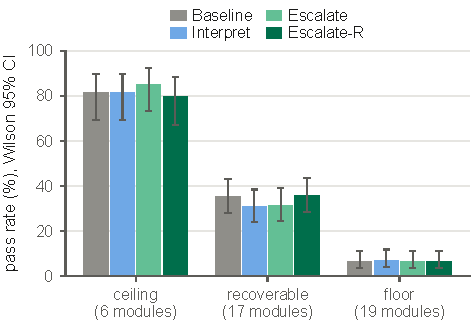
\includegraphics{fig_set1_tiers}
\caption{Pass rate by tier and condition}
\label{fig:set1-a}
\end{subfigure}\hfill
\begin{subfigure}[t]{3.15in}
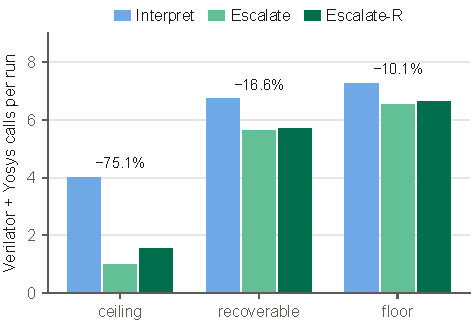
\includegraphics{fig_set1_calls}
\caption{Verilator and Yosys calls per run}
\label{fig:set1-b}
\end{subfigure}
\caption{Small open models (Gemma~3 4B, Llama~3.1 8B, DeepSeek-Coder 6.7B;
$1{,}512$ runs). (a)~The conditions differ only on the recoverable tier, and
there within noise. (b)~Escalation's cut in tool calls against \Interp{}
follows the tier: $75.1\%$ on the ceiling, $16.6\%$ on the recoverable tier,
$10.1\%$ on the floor.}
\label{fig:set1}
\end{figure}

\subsection{Larger Open Models and Commercial Models}
\label{sec:large}

On Qwen2.5-Coder 14B and 32B and Gemma~3 27B, the mean \Interp{} minus \Base{}
difference on the recoverable tier shrinks from $-4.6$ to $-0.65$ points, and
no condition differs from \Base{} (all $p \geq 0.40$). The nominal escalation
lead ($90/153$ against $86/153$) is not the interpreter at work: of the $65$
\Esc{} runs that escalated, the $2$ that passed did so without the interpreter
firing. Per model, the deficit is not monotonic in size (\cref{fig:ladder-b}):
Gemma~3 27B reverses it ($+7.8$) while Qwen2.5-Coder 32B keeps it ($-5.9$),
every interval crossing zero. The cost advantage, a mechanical count, grows:
escalation cuts tool calls by $27.6\%$ ($5.31$ to $3.85$ per run), because
capable models get stuck less often.

\begin{figure}[!htbp]
\centering
\begin{subfigure}[t]{3.15in}
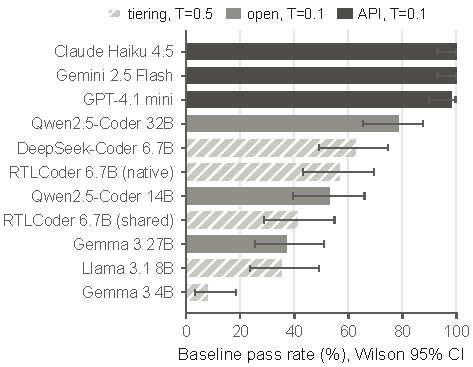
\includegraphics{fig_ladder}
\caption{\Base{} pass rate, every model}
\label{fig:ladder-a}
\end{subfigure}\hfill
\begin{subfigure}[t]{3.15in}
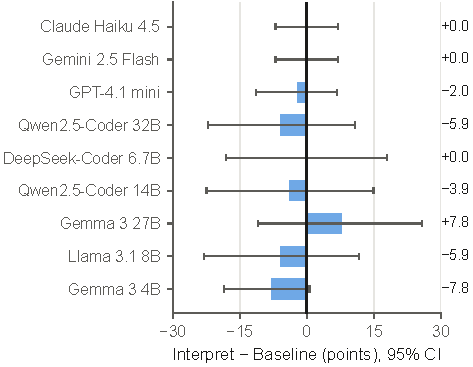
\includegraphics{fig_deficit}
\caption{Always-on interpretation minus \Base}
\label{fig:ladder-b}
\end{subfigure}
\caption{The capability ladder on the $17$ recoverable modules. (a)~\Base{}
pass rate for every model; the tiering-study bars ran at $T{=}0.5$, so the
ladder is ordinal across shades. (b)~The always-on deficit, with intervals for
a difference of two proportions~\cite{newcombe1998}, ordered by \Base{} pass
rate: small, not monotonic in model size, and every interval crosses zero.}
\label{fig:ladder}
\end{figure}

\paragraph{Commercial models} GPT-4.1 mini (snapshot 2025-04-14), Gemini~2.5
Flash (thinking budget $0$) and Claude Haiku~4.5 (no extended thinking) ran the
same protocol under a pre-registration, with a laptop toolchain that reproduced
the cluster's verdicts on $140$ saved candidates exactly. On the recoverable
tier they are at the ceiling ($98.0$ to $99.3\%$ in every condition): Gemini and
Haiku pass every run, and GPT-4.1 mini's tool conditions trail \Base{} by $2$
to $4$ points, all on one module, without significance. Escalation rarely
triggers, so its tool-call cut reaches $88.6\%$: up the capability ladder the
saving runs from $16.6\%$ through $27.6\%$ to $88.6\%$. Each passing module
cost INR~$0.11$ to $0.51$.

\subsection{The Floor Tier}
\label{sec:floor}

The commercial models also ran the $19$ floor modules, which no small open
model reliably passes. $16$ of them leave the floor under \Base{} for at least
one commercial model, so the floor is mostly a property of the $4$B to $32$B
models, not of the modules; only \texttt{adder\_pipe\_64bit}, \texttt{alu} and
\texttt{freq\_divbyfrac} stay at the floor for every model. On the remaining
failures the interpreter does fire, in $55\%$ of the failing runs under the
tool conditions, but no pass is attributable to it: only three passes followed
a directive in a cell whose \Base{} score was $0/3$, and traced individually,
none was caused by it. No condition differs significantly from \Base{}.

\paragraph{The one module every model fails: freq\_divbyfrac} Of the floor
modules all three commercial models ran, only this divide-by-$3.5$ clock divider
fails in every run ($0/36$). Its specification says that ``the counter cycles
through 7 half clock steps''; its reference design, which passes the testbench,
advances the counter once per rising edge and so wraps every $14$ half steps,
with two output periods per wrap. No final candidate is a phase-shifted copy of
the expected waveform; all $34$ that compile have about twice the specified
period. In our reading this is a specification defect, not a testbench defect,
and no interpreter can see it.

\subsection{Does Verilog Fine-Tuning Help? A Same-Base Comparison}
\label{sec:finetune}

RTLCoder-Deepseek-v1.1~\cite{rtlcoder,rtlcoder_hf} is DeepSeek-Coder 6.7B
fine-tuned on curated Verilog, so the pair isolates fine-tuning. On the
recoverable tier, at the shared prompt, RTLCoder passes $21/51$ against the base
model's $32/51$: no module wins, $13$ ties (at most one pass of three apart) and
$4$ losses, which trace to an undefined submodule, SystemVerilog-only syntax, a
parameter-binding failure and a memorised benchmark folder name used as the
module name. At its native prompt the comparison is a wash ($29/51$; $5$ wins,
$6$ ties, $6$ losses). Fine-tuning helps on one class: at its native prompt
RTLCoder clears every recoverable signal-processing module ($9/9$) and the
memory module ($3/3$). On this external benchmark, fine-tuning shows no net
advantage.

\paragraph{What RTLLM cannot show} RTLLM scores a module by its testbench alone,
and on its recoverable tier the interpreter had something to say in only about a
third of always-on runs ($52$ of $153$ for the small models): its modules rarely
contain defects that pass the testbench and break synthesis. Hand-written
hardware does.

% ============================================================================
\section{Case Study: A Hand-Written RISC-V MPSoC}
\label{sec:mpsoc}

\subsection{The Design, and Why It Is a Good Test}
\label{sec:mpsoc-design}

The MPSoC was written by hand within our group for an earlier project,
independently of this study, in an FPGA vendor flow (Vivado). Each node is a
five-stage RV32 core with instruction and data memories; a network interface
packs the core's traffic into flits and passes them through asynchronous FIFOs
to a router; and the routers form a mesh network-on-chip with virtual channels
and wormhole switching. The design exists as a $2{\times}2$ mesh ($4$ routers),
a $3{\times}3$ mesh ($9$ routers) and a processor top. We changed only what the
open-source tools refused to compile (duplicate declarations, nested comments,
implicit trailing ports), kept every connection identical, and touched no
defect.

\paragraph{How hand-written code hides sign-off defects} Module testbenches
exercise the intended behaviour, and an FPGA flow that infers a latch reports a
warning among hundreds and carries on. Pushed through Yosys, this design
reports $63$ latch inferences in $12$ module definitions and then aborts. Three
patterns recur, each natural to write. An incomplete \texttt{case} or
\texttt{if} in a combinational block (\cref{fig:motivation}): the forwarding
multiplexer \texttt{mem\_wb\_mux}, for instance, assigns its store-data output
only on some paths, so a latch holds a stale operand exactly in the cases the
testbench never applies. A register whose \texttt{always} block lists its
control signals instead of the clock edge (\texttt{always @(clr, ce)}), so
synthesis builds a latch where a flip-flop was meant. And a one-bit register
that tests \texttt{clr | reset} inside an asynchronous-reset block: it simulates
as intended, but synthesis cannot map a reset that depends on a synchronous
clear, and stops.

\paragraph{The defect at scale} One defective definition becomes many defective
cells. Every router instantiates two latching registers, of $32$ and $4$ bits,
$20$ times each, so the $2{\times}2$ mesh synthesises $2{,}880$ latch cells and
the $3{\times}3$ mesh $6{,}480$ (\cref{fig:compose-a}), while Yosys prints the
same two messages for both: the feedback a loop sees does not grow with the
damage. With the task modules repaired, both meshes synthesise with no latch;
the MPSoC top synthesises with $122$ latch cells left in five modules outside
the repair set, so its target is restored synthesis rather than a latch-free
design. The top-level testbench executes only two instructions, so claims about
composed designs are structural; functional claims rest on the module
testbenches.

\begin{figure}[!htbp]
\centering
\begin{subfigure}[t]{3.15in}
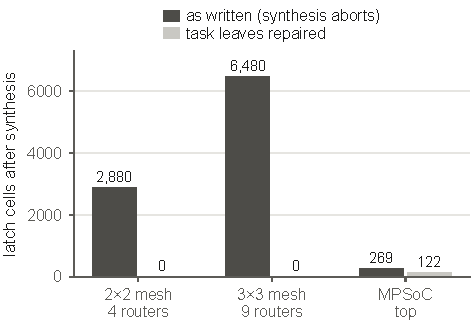
\includegraphics{fig_latch_scale}
\caption{The latch defect at scale}
\label{fig:compose-a}
\end{subfigure}\hfill
\begin{subfigure}[t]{3.15in}
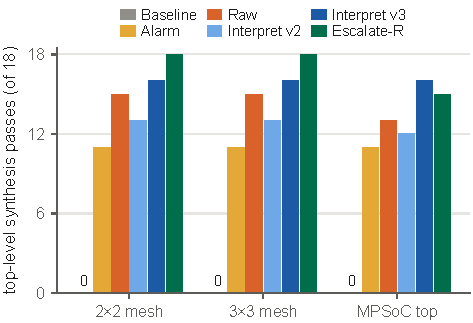
\includegraphics{fig_compose}
\caption{Top-level synthesis after repair, by condition}
\label{fig:compose-b}
\end{subfigure}
\caption{Leaf defects in the real designs. (a)~Latch cells grow with the router
count while Yosys prints the same two messages; with the task modules repaired,
both meshes have none. (b)~Each condition's repaired modules spliced back in
($18$ attempts per design: six models, three runs each).}
\label{fig:compose}
\end{figure}

\paragraph{Keeping the interpreter honest on real logs} On the real logs the
production interpreter (v2) showed gaps that synthetic tests had not: an unused
clock received the generic gating directive, which suggests \texttt{if (clk)}
and so builds a clock-gated latch, and the asynchronous-reset abort and an
expression truncation produced no directive at all. The v3 layer
(\cref{tab:rules}) adds rules only where a real log showed the production
directive wrong or missing; its key rule combines a Yosys latch with a
Verilator unused-clock warning into a missing-clock-edge diagnosis. A check that
runs the interpreter on fresh tool output before any GPU time caught a change in
Yosys's latch message between versions $0.33$ and $0.69$ that would otherwise
have silently disabled the new rules.

\subsection{Experimental Design}
\label{sec:mpsoc-exp}

\paragraph{Tasks} Eleven repair tasks (\cref{tab:tasks}): the eight defective
real leaves and three seeded modules for defect classes the design lacks. Six
are \emph{simulation-silent}: the defective module already passes its loop
testbench, so only lint or synthesis can reveal the defect. Specifications
describe behaviour only; with hints in them, a pilot $8$B model fixed every
defect on its first call under every condition.

\begin{table}[!htbp]
\centering
\footnotesize
\caption{The eleven repair tasks. Origin: R, a real leaf of the hand-written
design; S, seeded for a class the design lacks. A dot marks the two tasks
whose sign-off testbench checks more than the loop testbench.}
\label{tab:tasks}
\begin{tabular}{@{}l l l c l c@{}}
\toprule
Task & Role in the design & Defect, as written & Origin & Loop testbench & \makecell{Stricter\\sign-off} \\
\midrule
\texttt{MuxPC}            & next-PC select           & latch (incomplete \texttt{case}) & R & passes it & \\
\texttt{execute\_mux}     & ALU or multiplier result & latch                            & R & passes it & \\
\texttt{mux3}             & operand forwarding       & latch                            & R & passes it & \\
\texttt{mem\_wb\_mux}     & store-data forwarding    & latch                            & R & passes it & $\bullet$ \\
\texttt{register\_1bit}   & router state bit         & unmappable asynchronous reset    & R & passes it & \\
\texttt{riscv\_alu\_flags}& ALU with status flags    & latch on the flags               & S & passes it & \\
\addlinespace
\texttt{Address\_select}  & jump target, PC source   & latch, 1-bit \texttt{PC} port    & R & fails it  & $\bullet$ \\
\texttt{register\_32bit}  & router pipeline register & missing clock edge (latch)       & R & fails it  & \\
\texttt{register\_4bit}   & router channel state     & missing clock edge (latch)       & R & fails it  & \\
\texttt{noc\_xbar4}       & router crossbar port     & multi-driven output              & S & fails it  & \\
\texttt{ni\_flit\_pack}   & flit packer              & width truncation                 & S & fails it  & \\
\bottomrule
\end{tabular}
\end{table}

\paragraph{Conditions and runs} All six conditions share one budget of six model
calls, the same prompt and identically filtered raw tool text, and every run
starts from the defective module. \Base{} stops at the first simulation pass, as
AutoChip does, so on a simulation-silent task it stops at the input without
calling the model; that is exactly what a simulation-only loop does, and the
like-for-like comparison is on the simulation-visible tasks. \EscR{} opens with
the \Alarm{} message, escalates to v3 directives after two identical error
signatures, and may restart once. \Alarm{} gives the same opening message but
never escalates; what v3 would have said is logged, never fed back. Six open
models from 3B to 14B ran five conditions on the cluster ($990$ runs). The
\Alarm{} arm for them ($198$ runs) and Qwen2.5-Coder 32B under all six
conditions ($198$ runs) were \emph{pre-registered}: before any of their runs,
four primary contrasts and the reading each outcome would support were written
down and frozen with the runner, interpreter and task files. The three
commercial models ran all six conditions ($198$ runs each) and are reported per
model.

\paragraph{Two testbenches, and how a run is scored} Each task has a \emph{loop
testbench}, which drives feedback and stopping, and a
\emph{specification-complete sign-off testbench}, which scores the returned RTL
offline and never reaches the loop. The sign-off testbench was added after an
equivalence audit (Result~8) found two tasks whose loop testbench misses
specified behaviour; on the other nine the two are identical. Because the loop
never saw it, re-scoring the first $990$ runs is exact (post hoc for those runs,
pre-registered for the rest). A run is \textbf{sign-off clean}, the primary
metric, when the sign-off testbench passes, Yosys reports no latch or
combinational loop, and Verilator reports no multi-driven net, loop, latch or
truncation. It is \textbf{signed off defective} when the loop testbench passes,
so a simulation-only loop would accept it, but it is not sign-off clean. The
$198$ runs of a condition form $66$ (model, task) cells for the contrasts of
\cref{sec:stats}.

\subsection{Results}
\label{sec:mpsoc-results}

\paragraph{Result 1: simulation-only repair signs off defective RTL; with lint
and synthesis, latch-free clean synthesis on the latch-bearing tasks rises from
24\% to 88\%} On the eight latch-bearing tasks, $35$ of $144$ \Base{} runs end
latch-free with a clean synthesis, against $127$ of $144$ under \Ithree{} and
\EscR{} (\cref{fig:teaser-b}); \Itwo{} reaches $85\%$, \Raw{} $72\%$ and
\Alarm{} $65\%$. This count uses Yosys alone, so it depends on neither
testbench. \Base{} passes its loop testbench in $85\%$ of runs but is sign-off
clean in only $22\%$: $63\%$ of its runs are signed off defective
(\cref{tab:mpsoc-cond}), including all $108$ simulation-silent runs, and for
Qwen2.5-Coder 32B and each commercial model all $18$ simulation-silent runs are
too. With lint and synthesis in the loop, signed-off-defective runs fall to $8$
to $15\%$.

\begin{table}[!htbp]
\centering
\footnotesize
\caption{The MPSoC study by condition (six open models, $198$ runs each).
\EscR{} is sign-off clean most often; with any tool feedback, signed off
defective falls from $63\%$ to $8$ to $15\%$.}
\label{tab:mpsoc-cond}
\begin{tabular}{@{}l rcr r rr@{}}
\toprule
 & \multicolumn{3}{c}{Sign-off} & \multicolumn{1}{c}{Loop} & \multicolumn{2}{c}{Cost} \\
\cmidrule(lr){2-4}\cmidrule(lr){5-5}\cmidrule(l){6-7}
Condition & \makecell[r]{clean\\\%} & \makecell{95\%\\interval} & \makecell[r]{defective\\\%} & \makecell[r]{pass\\\%} &
  \makecell[r]{calls\\per run} & \makecell[r]{tokens\\per run} \\
\midrule
\sw{cBase}\ \Base     & 22 & 17--28 & 63 & 85 & 1.34 & 1,425 \\
\sw{cGate}\ \Alarm    & 52 & 45--59 & 15 & 67 & 3.39 & 3,835 \\
\sw{cRaw}\ \Raw       & 53 & 46--59 & 12 & 65 & 3.27 & 4,396 \\
\sw{cVtwo}\ \Itwo     & 63 & 56--69 & \textbf{8} & 71 & 2.83 & 3,831 \\
\sw{cVthree}\ \Ithree & 67 & 60--73 & \textbf{8} & 74 & 2.51 & 3,377 \\
\sw{cEsc}\ \EscR      & \textbf{72} & 65--78 & 13 & 85 & 2.99 & 3,798 \\
\bottomrule
\end{tabular}
\end{table}

\paragraph{Result 2: what the model is told decides the repair; the alarm alone
is not enough} Told only that sign-off failed, \Alarm{} reaches $52\%$ sign-off
clean, level with \Raw{} ($53\%$); interpretation reaches $63\%$ (v2) and $67\%$
(v3), and \EscR{} $72\%$. The pre-registered contrasts (\cref{tab:primary})
give the reading registered in advance for this outcome: \emph{the detail in
the feedback adds value beyond the verdict}. As registered, they carry no
multiplicity correction; under a Holm correction contrast~1 remains significant
and contrast~2 does not. Scoring with the loop testbench gives the same reading.
The alarm plateaus after the third call, while \EscR, which opens with the same
alarm, climbs from $56$ to $72\%$ once it hands over to v3 (\cref{fig:p3-b});
and the alarm alone breaks working logic: of $108$ simulation-silent \Alarm{}
runs, all starting from RTL that simulates correctly, $80$ still pass the loop
testbench at the end, against $97$ under \EscR. The gain is largest on the
smallest models: $39.4$ points on Llama~3.2 3B and $33.3$ on Gemma~3 4B, both
significant after correction.

\begin{figure}[!htbp]
\centering
\begin{subfigure}[t]{3.15in}
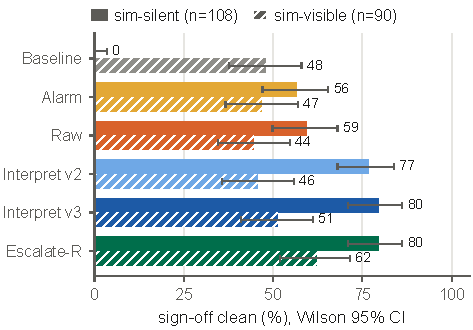
\includegraphics{fig_p3_stratum}
\caption{Sign-off clean by condition and task type}
\label{fig:p3-a}
\end{subfigure}\hfill
\begin{subfigure}[t]{3.15in}
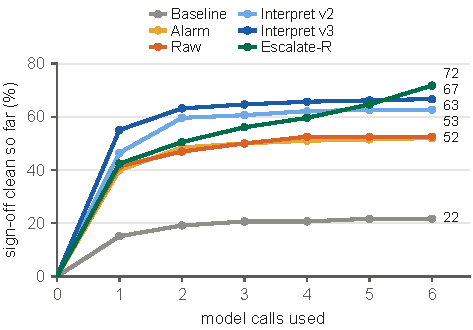
\includegraphics{fig_p3_bycall}
\caption{Sign-off clean after each model call}
\label{fig:p3-b}
\end{subfigure}
\caption{The MPSoC study, six open models. (a)~Simulation-only repair scores
$0/108$ on simulation-silent defects by construction; escalation leads on both
task types. (b)~v3 front-loads its repairs, the alarm alone plateaus after the
third call, and \EscR{} climbs to the highest final rate.}
\label{fig:p3}
\end{figure}

\begin{table}[!htbp]
\centering
\footnotesize
\caption{Pre-registered primary contrasts on sign-off clean (six open models):
difference in points, $95\%$ interval, $p$-value, and the runs that only A or
only B got right. Escalation and v3 beat the alarm; the alarm is no better than
raw text or simulation alone.}
\label{tab:primary}
\begin{tabular}{@{}l l S[table-format=+2.1] S[table-format=+2.1]@{\ to\ }S[table-format=+2.1] r r@{}}
\toprule
Contrast (A $-$ B) & Tasks & {$\Delta$} & \multicolumn{2}{c}{95\% interval} & $p$ & A/B only \\
\midrule
1. \EscR{} $-$ \Alarm & all & +19.7 & +11.1 & +29.3 & $<$0.001 & 42/3 \\
   & \quad simulation-silent  & +23.1 & +11.1 & +37.0 & 0.002 & 27/2 \\
   & \quad simulation-visible & +15.6 & +4.4  & +27.8 & 0.022 & 15/1 \\
\addlinespace
2. \Ithree{} $-$ \Alarm & all & +14.6 & +3.0 & +26.3 & 0.021 & 43/14 \\
   & \quad simulation-silent  & +23.1 & +6.5  & +39.8 & 0.014 & 31/6 \\
   & \quad simulation-visible & +4.4  & -11.1 & +20.0 & 0.688 & 12/8 \\
\addlinespace
3. \Alarm{} $-$ \Raw & all & -0.5 & -9.1 & +8.1 & 1.000 & 16/17 \\
4. \Alarm{} $-$ \Base & simulation-visible & -1.1 & -4.4 & +2.2 & 1.000 & 2/3 \\
\bottomrule
\end{tabular}
\end{table}

\paragraph{Result 3: interpretation beats raw text, sooner and more cheaply}
With the same raw text and budget, \Ithree{} is sign-off clean in $132$ of $198$
runs against \Raw's $104$: $+14.1$ points (interval $+3.5$ to $+24.7$). The
production interpreter, never tuned on these designs, gains $10.1$ points
(interval $+2.0$ to $+18.7$), the out-of-sample estimate. v3 needs about $23\%$
fewer model calls and tokens, and $55\%$ of its runs are sign-off clean after
the first call, against $41\%$ with raw text. The gain is largest where raw
text is hardest to use: $24.2$ points on Llama~3.2 3B and $27.3$ on
Qwen2.5-Coder 7B, while the 14B model is at $30/33$ either way.

\paragraph{Result 4: escalation reaches the highest sign-off-clean rate with the
fewest tool rounds} \EscR{} reaches $72\%$, keeps \Base's $85\%$ loop pass rate,
and uses $47.5\%$ fewer tool-feedback rounds than always-on v3. On the
simulation-visible tasks, where \Base{} does run the model, \EscR{} beats it by
$14.4$ points ($56/90$ against $43/90$, interval $+3.3$ to $+27.8$), and it
protects the smallest model: Llama~3.2 3B is sign-off clean there in $7/15$ runs
with simulation only, $1/15$ with raw text on every round, and $8/15$ with
escalation.

\paragraph{Result 5: repaired leaves let the real designs synthesise} With each
(model, run) set of repaired leaves spliced back (\cref{fig:compose-b}),
simulation-only repair never yields a design that synthesises, because it never
touches the simulation-silent register that aborts synthesis. \Ithree{}
succeeds in $16$ of $18$ attempts per design, and \EscR{} in $18$ of $18$ for
both meshes and $15$ of $18$ for the MPSoC top. Whenever every composed leaf was
clean, the design reached its target ($32/32$, $32/32$, $27/27$).

\paragraph{Result 6: up the ladder, any tool feedback suffices, but the guard is
still needed} For Qwen2.5-Coder 32B and the three commercial models
(\cref{tab:ladder}), any tool feedback repairs every simulation-silent defect,
so interpretation's edge vanishes; almost every remaining miss is on
\texttt{Address\_select} (Result~8). Yet simulation-only repair still signs off
all $18$ simulation-silent runs as defective for every model: the pass-rate
benefit is a small-model effect, but the guard is needed at every size.

\begin{table}[!htbp]
\centering
\footnotesize
\caption{Larger and commercial models in the MPSoC study, reported per model:
sign-off clean on the simulation-silent tasks (sil., of $18$) and the
simulation-visible tasks (vis., of $15$), and tokens per run (tok.). Any tool
feedback repairs every simulation-silent defect; simulation alone repairs none.}
\label{tab:ladder}
\setlength{\tabcolsep}{3.2pt}
\begin{tabular}{@{}l rrr@{\hspace{11pt}}rrr@{\hspace{11pt}}rrr@{\hspace{11pt}}rrr@{}}
\toprule
 & \multicolumn{3}{c}{Qwen2.5-Coder 32B} & \multicolumn{3}{c}{GPT-4.1 mini} & \multicolumn{3}{c}{Claude Haiku 4.5} & \multicolumn{3}{c}{Gemini 2.5 Flash} \\
\cmidrule(lr){2-4}\cmidrule(lr){5-7}\cmidrule(lr){8-10}\cmidrule(l){11-13}
Condition & sil. & vis. & tok. & sil. & vis. & tok. & sil. & vis. & tok. & sil. & vis. & tok. \\
\midrule
\Base     & 0  & 12 & 663   & 0  & 12 & 440   & 0  & 12 & 517   & 0  & 15 & 516 \\
\Alarm    & 16 & 12 & 1,824 & 16 & 12 & 1,529 & 18 & 12 & 1,099 & 18 & 15 & 1,160 \\
\Raw      & 18 & 12 & 1,492 & 18 & 12 & 1,164 & 18 & 12 & 1,334 & 18 & 12 & 1,291 \\
\Itwo     & 18 & 12 & 1,655 & 18 & 12 & 1,255 & 18 & 12 & 1,517 & 18 & 15 & 1,478 \\
\Ithree   & 18 & 12 & 1,660 & 18 & 12 & 1,257 & 18 & 12 & 1,524 & 18 & 14 & 1,479 \\
\EscR     & 18 & 12 & 1,850 & 18 & 12 & 1,404 & 18 & 12 & 1,101 & 18 & 15 & 1,225 \\
\bottomrule
\end{tabular}
\end{table}

\paragraph{Result 7: the v3 upgrade closes the vocabulary gaps} Where v2 was
silent (the asynchronous-reset register, the flit packer's truncation), v3
fires the intended rule in $18$ of $18$ runs, and where v2 misled (the two
latching registers, the address selector) it gives the right directive. On the
asynchronous-reset register, whose abort blocks synthesis of both meshes,
interpreter-credited repairs rise from $3/18$ to $15/18$. Across the four tasks
singled out before the runs, sign-off clean rises from $42/72$ to $50/72$
(interval $-9.7$ to $+31.9$ points): a favourable direction that remains
in-sample, since the v3 rules were written from these designs' logs.

\paragraph{Result 8: oracle integrity, and a limitation of structural advice}
Every repair in the first $990$ runs that passed its loop testbench with a clean
synthesis was checked against the golden fix by formal equivalence in Yosys.
Two loop testbenches proved incomplete. In \texttt{mem\_wb\_mux} the original
latch had held a stale store operand in exactly the cases the testbench never
applies, and $16$ repairs drive an unspecified value there. In
\texttt{Address\_select} the specification defines \texttt{J\_addr} $= X +
\texttt{PC}$ on every input, the testbench checks it only on a non-flushed jump,
and $41$ repairs set \texttt{J\_addr} to $0$ elsewhere: latch-free and
synthesisable, yet in violation of the specification. The production latch
directive suggests ``one unconditional assignment at the top of the block'' of
the form \texttt{J\_addr = <safe value>}; that advice reached every such run
under \Itwo, \Ithree{} and \EscR{} ($8$, $12$ and $11$), while \Base, \Raw{} and
\Alarm{} produced $3$, $7$ and $2$ without it: a count, not a causal claim. A
structural fix can be functionally wrong exactly where the loop testbench does
not look, and a specification-complete sign-off oracle catches it.

\paragraph{What the case study establishes} On real multiprocessor RTL a
simulation-only loop is blind to sign-off at every model size. Being told
\emph{that} sign-off failed is worth about as much as raw tool text; being told
\emph{what} failed adds $14.6$ points through interpretation and $19.7$ through
escalation; and fixing a handful of module definitions restores synthesis of
networks with $4$ and $9$ routers.

% ============================================================================
\section{Threats to Validity}
\label{sec:threats}

\runin{Statistical} Runs of a cell are correlated, so general claims rest on
cell-level intervals; three runs leave the small-model deficit and several
per-model effects undecided; and the primary contrasts carry no multiplicity
correction (under Holm, only contrast~1 survives). \runin{Sampling} One
temperature per study and quantised local models; the
\Alarm{} arm ran on a different inference backend (Vulkan, not CUDA), with no
detectable effect on byte-identical prompts. \runin{Toolchains} Diagnostic
formats change between versions; a live check caught one change.
\runin{In-sample interpreter} The v3 rules were written from the MPSoC's logs;
v2's out-of-sample gain is the conservative estimate. \runin{Oracle} The
sign-off testbench is post hoc for the first $990$ MPSoC runs; the loop
testbench gives the same reading. \runin{Benchmark} RTLLM is public, which may
inflate commercial models' absolute rates but not comparisons within a model.
\runin{Coverage} Claude Haiku~4.5 is incomplete on the floor tier.
\runin{Drift} Hosted models change behind stable names; we pinned snapshots
where possible. \runin{Composition} Composed
designs were checked by synthesis, not simulated. \runin{Scope} No timing
analysis or test insertion was run.

% ============================================================================
\section{Conclusion and Directions}
\label{sec:conclusion}

STITCH's conference version showed, one run at a time, that an interpreter can
help. On replicated evidence the picture is narrower and more useful. On a
testbench-scored benchmark the interpreter acts only on defects it can reach,
and escalation with a restart matches \Base{} while saving more tool calls the
stronger the model. On real hardware, STITCH is best read as a deterministic
sign-off guard and translator: it catches what simulation misses at every model
size, its detail rather than its alarm drives repair, and the repaired leaves
restore synthesis of whole designs, at no inference cost of its own.

\paragraph{Directions} (i)~Held-out real defects, to test the v3 rules out of
sample. (ii)~A latch directive that defaults each signal to the value the
specification defines, not to a constant. (iii)~Feedback for defects that exist
only once modules are connected, such as the MPSoC's one-bit program-counter
port driven with $32$ bits. (iv)~Reasoning models, which this study does not
cover. (v)~Specification-level robustness: in \texttt{freq\_divbyfrac} the
specification and its reference disagree, a defect no interpreter can see.

% ============================================================================
\section*{Availability}
Code, runners, analysis scripts, pre-registrations and evidence reports are at
\url{https://github.com/Karthik-Flash/STITCH}. Per-run logs are available on
request.

\section*{Acknowledgments}
This work is partially supported by the research project sponsored by
Xilinx-AMD. Opinions and conclusions presented are solely those of the authors
and are not representative of AMD's roadmap. The cluster runs used the
institutional high-performance computing facility of BITS Pilani, Hyderabad
Campus.

% ============================================================================
\begin{thebibliography}{99}
\footnotesize
\setlength{\itemsep}{0pt}

\bibitem{stitch26}
K.~Patana, Y.~Rajesh, A.~Sunil, D.~Saranyu, S.~Parameswaran, K.~Chandrasekar,
P.~Saxena, and S.~Joshi, ``STITCH: Semantic Toolchain Integration for
LLM-Driven RTL Circuit and Hardware Design Generation,'' in \emph{Proc. ACM/IEEE
MLCAD}, 2026, doi:10.1145/3831599.3840333.

\bibitem{cummings1999}
C.~E.~Cummings, ``\texttt{full\_case parallel\_case}, the Evil Twins of Verilog
Synthesis,'' in \emph{Proc. Synopsys Users Group Conference (SNUG)}, Boston,
1999.

\bibitem{autochip}
S.~Thakur, J.~Blocklove, H.~Pearce, B.~Tan, S.~Garg, and R.~Karri, ``AutoChip:
Automating HDL Generation Using LLM Feedback,'' arXiv:2311.04887, 2023.

\bibitem{rtlfixer}
Y.~Tsai, M.~Liu, and H.~Ren, ``RTLFixer: Automatically Fixing RTL Syntax Errors
with Large Language Model,'' in \emph{Proc. DAC}, 2024,
doi:10.1145/3649329.3657353.

\bibitem{verilogeval}
M.~Liu, N.~Pinckney, B.~Khailany, and H.~Ren, ``VerilogEval: Evaluating Large
Language Models for Verilog Code Generation,'' in \emph{Proc. ICCAD}, 2023,
doi:10.1109/ICCAD57390.2023.10323812.

\bibitem{lu2024rtllm}
Y.~Lu, S.~Liu, Q.~Zhang, and Z.~Xie, ``RTLLM: An Open-Source Benchmark for
Design RTL Generation with Large Language Model,'' in \emph{Proc. ASP-DAC},
2024, doi:10.1109/ASP-DAC58780.2024.10473904.

\bibitem{rtlcoder}
S.~Liu, W.~Fang, Y.~Lu, Q.~Zhang, H.~Zhang, and Z.~Xie, ``RTLCoder:
Outperforming GPT-3.5 in Design RTL Generation with Our Open-Source Dataset and
Lightweight Solution,'' in \emph{Proc. IEEE LLM Aided Design Workshop (LAD)},
2024, doi:10.1109/LAD62341.2024.10691788.

\bibitem{rtlcoder_hf}
RTLCoder-Deepseek-v1.1, Hugging Face model repository.
\url{https://huggingface.co/ishorn5/RTLCoder-Deepseek-v1.1}

\bibitem{selfrefine}
A.~Madaan et~al., ``Self-Refine: Iterative Refinement with Self-Feedback,'' in
\emph{Advances in Neural Information Processing Systems 36 (NeurIPS)}, 2023.

\bibitem{qiu2024}
S.~Qiu, B.~Tan, and H.~Pearce, ``LLM-aided Explanations of EDA Synthesis
Errors,'' in \emph{Proc. IEEE LLM Aided Design Workshop (LAD)}, 2024,
doi:10.1109/LAD62341.2024.10691721.

\bibitem{verilogcoder}
C.-T.~Ho, H.~Ren, and B.~Khailany, ``VerilogCoder: Autonomous Verilog Coding
Agents with Graph-based Planning and Abstract Syntax Tree (AST)-based Waveform
Tracing Tool,'' in \emph{Proc. AAAI}, 2025, doi:10.1609/aaai.v39i1.32007.

\bibitem{mage}
Y.~Zhao, H.~Zhang, H.~Huang, Z.~Yu, and J.~Zhao, ``MAGE: A Multi-Agent Engine
for Automated RTL Code Generation,'' in \emph{Proc. DAC}, 2025,
doi:10.1109/DAC63849.2025.11133191.

\bibitem{aivril}
M.~ul~Islam, H.~Sami, P.-E.~Gaillardon, and V.~Tenace, ``AIvril: AI-Driven RTL
Generation With Verification In-The-Loop,'' arXiv:2409.11411, 2024.

\bibitem{meic}
K.~Xu et~al., ``MEIC: Re-thinking RTL Debug Automation using LLMs,'' in
\emph{Proc. ICCAD}, 2024, doi:10.1145/3676536.3676801.

\bibitem{uvllm}
Y.~Hu et~al., ``UVLLM: An Automated Universal RTL Verification Framework using
LLMs,'' arXiv:2411.16238, 2024.

\bibitem{deepseekcoder}
D.~Guo et~al., ``DeepSeek-Coder: When the Large Language Model Meets
Programming -- The Rise of Code Intelligence,'' arXiv:2401.14196, 2024.

\bibitem{gemma3}
Gemma Team, ``Gemma 3 Technical Report,'' arXiv:2503.19786, 2025.

\bibitem{llama3}
A.~Grattafiori et~al., ``The Llama 3 Herd of Models,'' arXiv:2407.21783, 2024.

\bibitem{qwen25coder}
B.~Hui et~al., ``Qwen2.5-Coder Technical Report,'' arXiv:2409.12186, 2024.

\bibitem{iverilog}
S.~Williams, ``Icarus Verilog.'' \url{https://steveicarus.github.io/iverilog/}

\bibitem{verilator}
W.~Snyder, ``Verilator.'' \url{https://www.veripool.org/verilator/}

\bibitem{yosys}
C.~Wolf, ``Yosys Open SYnthesis Suite.'' \url{https://yosyshq.net/yosys/}

\bibitem{ollama}
Ollama. \url{https://ollama.com}

\bibitem{wilson1927}
E.~B.~Wilson, ``Probable Inference, the Law of Succession, and Statistical
Inference,'' \emph{J. Amer. Statist. Assoc.}, vol.~22, no.~158, pp.~209--212,
1927, doi:10.1080/01621459.1927.10502953.

\bibitem{newcombe1998}
R.~G.~Newcombe, ``Interval Estimation for the Difference Between Independent
Proportions: Comparison of Eleven Methods,'' \emph{Statistics in Medicine},
vol.~17, no.~8, pp.~873--890, 1998.

\end{thebibliography}

\end{document}
